%!TEX program = xelatex
\documentclass[UTF8]{article}
\usepackage{graphicx}
\usepackage{setspace}
% \usepackage{ctex}
\usepackage{indentfirst}
\setlength{\parindent}{2em}  % 用于首行缩进

\usepackage{amsmath}
\usepackage{amsthm} % 使用定理环境
\usepackage{amssymb}

\usepackage[colorlinks,linkcolor=red,anchorcolor=blue,citecolor=green,CJKbookmarks=True]{hyperref}  % 使用链接 但不用默认属性
% CJKbookmarks让链接支持中文
% \usepackage{hyperref}
% \usepackage{geometry}
% \geometry{a4paper,scale=0.8}
\usepackage{algorithm}
\usepackage{algorithmic}
\usepackage{geometry}
\geometry{a4paper,left=2.0cm,right=2.0cm,top=3.0cm,bottom=3.0cm}
\setstretch{1.5}   %  改变行间距
% \newgeometry{left = 2 cm, top= 3 cm}

\title{Summary}
\author{Dis\cdot count}
% \date{Feb 2019}

% \newtheorem{algorithm}{Algorithm}
\newtheorem{thm}{\hspace{2em}Theorem}
\newtheorem{lem}{\hspace{2em}Lemma}
\newtheorem{pf}{\hspace{2em}Proof}
\newtheorem{remark}{\hspace{2em}Remark}
%  \newtheorem{def}{Definition}  doesnt work


\begin{document}

\maketitle{}

\section*{Abstract}



Keywords: Cooperative game, scheduling, pricing for coopration.


In this paper, instead of sacrificing the entrepreneur’s profits, we are interested in motivating early investors by reallocating final profits earned from the proposal. Intuitively, we assign more profits to early investors so that their waiting costs are balanced out and the resulting pledging probabilities are raised. Note that more profits allocated to (higher pledging probabilities of) early investors means less profits remain for (lower pledging probabilities of) the late ones. To enhance the overall success rate of a crowdfunding project, it is of utmost importance to provide the entrepreneur with appropriate profit allocation mechanisms. Our main contributions are summarized as follows.
First, to the best of our knowledge, this paper is the first attempt to analytically study the profit
allocation mechanism to enhance the success rates of investment-based crowdfunding projects. Most
literature on crowdfunding, especially investment-based crowdfunding, is empirical and existing efforts
on motivating investors focus on offering additional benefits and price discounts. Our study helps the entrepreneur design an optimal profit allocation mechanism to maximize the success rate without sacrificing the profits of the entrepreneur.
Second, we develop static models to analyze the pledging behavior of investors, and we characterize
the “waiting cost” to explain the inequity between investors at different stages in crowdfunding projects. The main results show that because of the waiting cost, investors who arrive early are less willing to pledge money. It also shows that the entrepreneur should motivate early investors to enhance the success rate of the project. In addition, the extra return given to early investors as an incentive should increase with the waiting cost.
Third, as a generalization, we consider the difference in the number of investors who group as cohorts, arriving at different points in time. We find that investors in different-sized cohorts are not equally sensitive with changes in profit allocation, and the entrepreneur should motivate investors in smaller cohorts to enhance the success rate of his crowdfunding project. This property, together with the effect of the waiting cost, decides the profit allocation strategy of the entrepreneur. In addition, we also provide managerial guidance on how the entrepreneur should adjust the optimal profit allocation mechanism when other factors in the market change.
三方面贡献,首先最重要的 是提出 pricing 的概念, 这个概念不同于已有的 惩罚和补贴; 提出概念之后建立了相应的模型,并且提出了相应的解法,归到一个可以求解的问题; generalization, 对于有权重的部分也可用类似的方法,得到了能这样求解的一般性质;
pricing 对于政府定价有一定的启示.

以及第七的拓展部份 提到 pricing 会有固定的两/三个价格提供稳定

The rest of this paper is structured as follows. The following section reviews relevant literature. We describe the basic problem in Section 3. In Section 4, we analyze the profit allocation mechanism using a
primary model where there are only two potential investors. Section 5 generalizes the results of Section 4 by studying a two-cohort model where there are two cohorts of investors. The conclusions are shown in Section 6.


\section*{Introduction}

At first, we will introduce some preliminary knowledge about cooperative game theory as follows.
A pair $(V,c)$ is usually used to represent a cooperative game with transferable utilities, among which $V=\{1,2,\dots,v\}$ denotes a set of $v$ players and $c:2^{V}\to \mathbb{R}$ indicates the characteristic function of the game. A coalition $s$ is defined as a non-empty subset of players; and $V$ is refered to as the grand coalition containing all the players, $S=2^{V} \setminus\{\emptyset\}$ denotes the set of all feasible coalitions. The characteristic function of the game, $c(s)$, represents the minimum coalitional cost the players in $s$ have to pay in order to cooperate together.
A cost allocation vector $\alpha=[\alpha_{1},\alpha_{2},\dots,\alpha_{v}] \in \mathbb{R}^{v}$ is required by the game to maintain cooperation in the grand coalition, and $\alpha_{k}$ is the cost assigned to players $k \in V$ to assure no individual or group of players has the incentive to deviate. For the convenience of abbreviation, we use $\alpha(s)=\sum_{k\in{s}}\alpha_{k}$ to denote the total cost assigned to the players in coalition $s$.
One of the most important concepts in cooperative game theory is core, which is a cost allocation satisfying two kinds of contraints, one is the budget balance contraint {$\alpha(V)=c(V)$} and the other is the coalitional stability constraints {$\alpha(s) \leq c(s)$}. In other words, core can be expressed as

\[
Core(V,c)= \left\{\alpha:\alpha(V)=c(V), \alpha(s)\leq c(s)\ \text{for all}\ s \in S \setminus\{V\}, \alpha \in \mathbb{R}^{v} \right\}.
\]

When the cost allocation exists, core is called non-empty. And if and only if the core is non-empty, the grand coalition of the associating cooperative game $(V,c)$ will be stable or balanced.

However, cooperative games can be unbalanced in many cases owing to the joint restrictions of the above-mentioned two kinds of constraints. To stabilize the grand coalition in unbalanced cooperative games, researchers have already developed several effective instruments, such as subsidization, penalization and simultaneously subsidization and penalization. The
similarity of these instruments is that there exists an outside party who will take measures to stabilize the grand coalition. But the penalization will always arouse the discontent of players in coalitions, it is promising to find a new instrument to replace the penalization, we call it pricing.
The significant idea of this instrument is that we can erase the role of the third party by collecting pricing as subsidy of the corresponding coalitions.
That being said, the players of the games can stabilize themselves without the third party.

To make the project concrete, we will apply this instrument on the machine scheduling games to show our ideas.


%\section{Outline}

For the effective domain $[0, P^*]$, we just need to divide this interval into several parts and the points are denoted as $P_L(V,i), i = 1,2,\ldots,n$.  At first, we don't need to calculate the initial part because this part the corresponding subsidy is 0 always. Then we just need to focus on the latter part which shows some interesting properties we proved above.

For any P in $[0, P^*]$, calculate the subsidy and the corresponding slope (Please refer to Liu et.al.2018) z

Flow path: IPC algorithm, (4q-1)

1-\sum_{s\in S\subset\{V\}} \rho_s

To follow the CP approach(Algorithm 3) to calculate the weak derivative, then use Algorithm 1 to obtain the subsidy \omega(z).

Questions: how to solve the LP(9) and the DP program.



% 这里还需要定义一个优化问题

\section*{Definition 0.}
In an Identical Alternative Parallel machine scheduling of Unweighted jobs (IAPU) game, each player $k$ in $V=\{1,2,\ldots,v\}$ has a job $k$ that needs to be processed on one of identical machines in $M=\{1,2,\ldots,m_v\}$, where $m_v$ is a given positive integer no more than $v$. Meanwhile, each machine has a setup cost $T$. Each job $k\in V$ has a processing time denoted by $t_k$. Each coalition $s \in S$, where $S=2^V\setminus\{\emptyset\}$, aims to schedule the jobs in $s$ on all machines in $M$ so that the total completion  time of the jobs in $s$ is minimized, i.e., to minimize $\sum_{k\in s}{C_k}+m_sT $,
where $C_k$ is the completion time of job $k\in s$.

% 暂且用T-i表示机器调度里的定价,等后期确定后再统一改。

Then we will illustrate the taxation instrument with a simple example of an IAPU game as follows.

\section*{Example}

There is an IPU game which contains four players, whose processing times on the identical parallel machine are $t_1=2, t_2=3, t_3=4, t_4=5$ respectively. Each machine setup cost is $t_0=9.5$, and $c(s)$ is the minimum total completion time of jobs in coalition $s$ plus the machine setup cost.

In this example, the grand coalition has a minimum cost, which is $c(V) = \sum_{k\in v}{C_k}+m_vT = 38$, and the optimum number of machine is $m_v = 2$.
It's easy to check that this example is unbalanced and calculate the subsidy which equals $c(V) - \alpha(V) = 0.75$.

When the setup cost increases from 9.5 to 13, that is, the taxation increases from 0 to 3.5,
the number of machine will decrease from 2 to 1, accordingly.

Although this case is easily understood, it demonstrate the concept of taxation we have strong interests in. Then we will define the corresponding model to further elaborate on this concept.

\section*{Definition 1.}

A cooperative TU game $(V,c)$ is called an AIPU game if it satisfies the following formulations.

\[
\begin{aligned}
c(s,P) = & {\min} \sum_{k\in V}\sum_{j\in O} {c_{kj} x_{kj}} + {P\sum_{k\in s} x_{k1}} \\
{s.t.}\quad & \sum_{j \in O} x_{kj}-y_k^s=0, \forall k \in V, \\
& \sum_{k\in V} x_{kj} \leq m,\forall j \in O,  \\
& x_{kj} \in \{0,1\} , \forall k \in V, \forall j \in O,\\
& y_k^s=1, k \in s, y_k^s=0, k \notin s.
\end{aligned}
\]
Among these formulations, $P$ and $m$ denotes the price and the number of using machines, respectively.
Now we've already extended the number of players to a more complex case, that is, the number of players is set to $n$.
Let $N=\{1,2,\ldots,n\}$ be a set of n players. The number of machines is $m$ and the setup cost is $P$.
For convenience of expression, we set the processing times $t_i(i\in N)$ satisfy $t_1<t_2<\cdots<t_n$.

Then we need to define two functions, practical subsidy-price function (PSPF) and theoretical subsidy-price function (TSPF) denoted by $\omega(P)$ and $\hat{\omega}(P)$, respectively:
\[
  {\omega(P)}=\mathop{\min}_{\alpha}\{c(V,m(V,P))-\alpha(V): \alpha(s)\leq c(s,m(s,P))
 ,\forall s \in S, \alpha\in\mathbb{R}^{v}\},
\]
\[
  {\hat{\omega}(P)}=\mathop{\min}_{\alpha}\{c(V,m(V,P))-\alpha(V): \alpha(s)\leq c(s,m(s,P))
 ,\forall s \in S\setminus\{V\}, \alpha\in\mathbb{R}^{v}\}.
\]

By dividing the PSPF function into two parts like $c(s)=c_0(s)+m(s)P, s \in S$, as a common skill, we can obtain its dual:
\begin{equation}\label{dual}
 {\omega^*(P)}=\mathop{\max}_{\rho} \{c_0(V)+m(V)P+\sum_{s\in S\setminus\{V\}}-\rho_s[c_0(s)+m(s)P]:
 \sum_{s\in S\setminus\{V\}:k\in s}\rho_s=1,\forall k \in V,\rho_s\geq 0,\forall s \in S \setminus{V}\}
\end{equation}

Then we need to define an interval $[P_L(m,s),P_H(m,s)]$ to denote the value range of price when the number of using machines $m$ and the coalition $s$ are given.

\begin{remark}
  It's easy to know that $P_L(m,s) = P_H(m+1,s)$, for each $s \in S$ and $ m <|s|$.
\end{remark}

\begin{remark}
  For the grand coalition $V$, we define $P_L(v,V) = 0, P_H(1,V) = P^*$. So the practical domain of the price is $[0,P^*]$ which is divided into $v$ parts by the number of using machines.
\end{remark}

\begin{remark}
  Note that $P_L(m,s) = P_H(m+1,s)$, for the sake of brevity and readability, we use $P_{m+1}$ to substitute for $P_L(m,s)$ or $P_H(m+1,s)$ later on.

\end{remark}

We can establish Theorem 1 below, showing the property of the function.

\begin{thm}\label{thm1}
$\omega(P)$ is piecewise linear, and convex in price P at each subinterval $[P_L(m,V),P_H(m,V)]$ in $[0,P^*] $.
\end{thm}


In this situation, the interval size of setup cost can be calculated when $t_i$ is known. And we can obtain that under what circumstances the machine number will change. We set the different intervals where the number of machines remain unchanged as $I_i$ respectively. The extreme points of these intervals are recorded as $P_i$ respectively, which represents the price when the number of using machine changes from $i$ to $i-1$. Specially, $P_1$ denotes the extreme point of the whole interval, which is the value of price or setup cost when using one machine and subsidy equals zero.

Note that the costs of all the exponential coalitions can be easily calculated by the SPT rules, we have Lemma \ref{lem1}.

\begin{lem}\label{lem1}

The value at the extreme points of the sub-intervals $I_i$ can be calculated with processing times $t_i$ by comparing the costs of the grand coalitions where all the players use two adjacent numbers of machines.
\end{lem}

According to the above lemma \ref{lem1}, we can obtain all the extreme points of the sub-intervals, i.e. , the number of using machines decreases by one when the price or setup cost equals $P_i$.


\begin{thm}\label{thm2}

According to the foregoing description, we have the equation $S_{1}=S_{2}+\cdots+S_{n}=\sum_{i=2}^n S_i$.

\end{thm}

With Theorem \ref{thm2}, we obtain all the breakpoints during the interval of the price where the machine number changes and the subsidy is $0$. Then we'll focus on the specific property of subsidy.

\begin{thm}\label{thm3}

The subsidy is always zero when the number of using machines, m, is larger than $\frac{n}{2}$.

\end{thm}

In other words, when the numbers of machine is larger than half of players, the grand coalition does't need any subsidy from the externality.

\begin{thm}\label{thm4}
The sum of absolute values of slopes at both sides of $S_i$ is 1.
When the number of machines used is 1, the range of slopes of the line segments in the interval is $\left( -1 , -\frac{1}{n-1} \right]$, and the number of breakpoints is $ O(v^2) $.
\end{thm}

Until here, we described the main property of the whole figure.
And a diagram of the number of machines and subsidy on setup cost, with its essential features being showed below.

\begin{figure}[h]%%图
	\centering  %插入的图片居中表示
	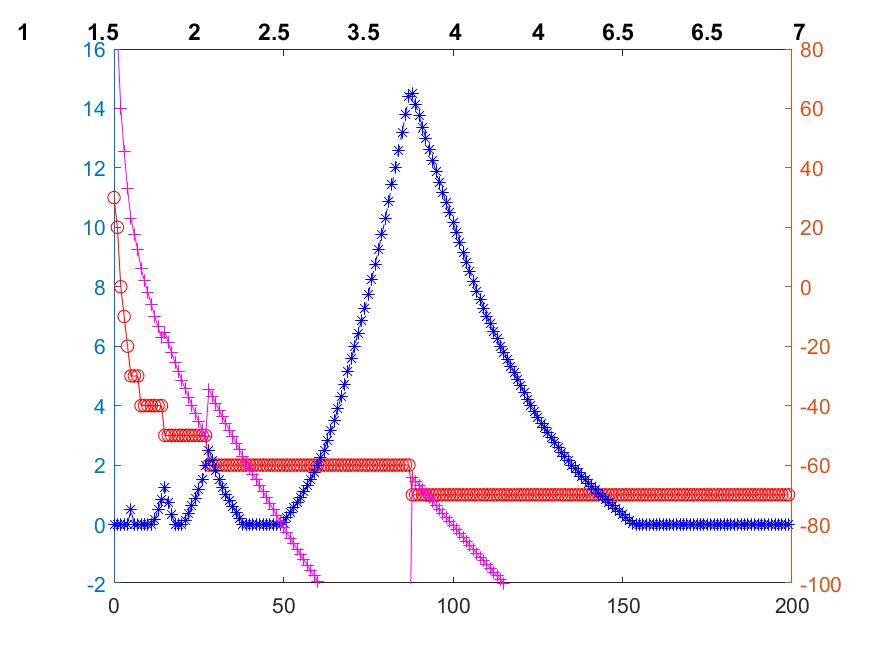
\includegraphics[width=0.8\linewidth]{Figures/Image30}  %插入的图,包括JPG,PNG,PDF,EPS等,放在源文件目录下
	\caption{The number of machines and subsidy on setup cost.}  %图片的名称
	\label{fig:Image11}   %标签,用作引用
\end{figure}

The processing times of all players with the arrangement from small to large are listed on the top of this figure.
The red and blue lines stand for the machine number and subsidy, respectively.
The horizontal ordinate represents the price or setup cost.
The left ordinate represents the value of machine number,while the right represents the value of subsidy.

As the coalitional stability constraints showed above, the exponential inequality constraints are so tricky that we must figure out a method to simplify these constraints to obtain the optimal results. Fortunately for us, we find the Theorem \ref{thm5}.


\begin{thm}\label{thm5}
The original problem is equivalent to using only one machine for all coalitions.

\end{thm}

By establishing the Theorem 5, we can design the specific algorithm to eliminate the redundant inequalitie, which will save us from the trouble of solving $c(s)$ and speed up the solution.

At first, we need to construct the PSPF function, which is piecewise linear and convex at every subinterval. If we can obtain the specific subsidy value $\omega(P)$ given any $P$, then we can calculate the breakpoints during the interval by IPC algorithm.

At first, we need to divide the interval into $n$ subintervals according to the  number of using machine of the grand coalition, at each subinterval we use the IPC algorithm to get the breakpoints. After applying the algorithm to all subintervals, we can obtain the PSPF function.


\begin{algorithm}[h]\label{algoIPC}
\caption{The Intersection Points Computation(IPC) Algorithm to Construct the PSF Function.}
\begin{algorithmic}[1]

\begin{description}
  \justifying
  \item[Step 1.] Initially, set $I^*=\{P_L,P_H\}$ and $\mathbb{I}= \{[P_L,P_H]\}$.
  \item[Step 2.] If $\mathbb{I}$ is not empty, update $I^*$ and $\mathbb{I}$ by the following steps:
  \item[Step 3.] Sort values in $I^*$ by $P_0<P_1<\cdots<P_q$, where $P_0 = P_L,P_q = P_H$ and $q = |I^*|-1$.
  \item[Step 4.]
  Select any interval from $\mathbb{I}$, denoted by $[P_{k-1},P_{k}]$ with $1\leq k \leq q$
  \item[Step 5.]
  Construct two linear function $ R_{k-1}(P)$ and $ L_{k}(P)$ so that $ R_{k-1}(P)$ passes $(P_{k-1},\omega(P_{k-1}))$ with \\
  \vspace{10pt}
  a slope equal to a right derivative $K_{r}^{P_{k-1}}$ of $\omega(P)$ at $P_{k-1}$, and that $L_{k}(z)$ passes $(P_{k},\omega(P_{k}))$ with a \\
  \vspace{10pt}
  slope equal to a left derivative $K_{l}^{P_{k}}$
  of $\omega(P)$ at $P_k$.
  \item[Step 6.] If $R_{k-1}(P)$ passes $(P_{k},\omega(P_{k}))$ or $L_{k}(P)$ passes $(P_{k-1},\omega(P_{k-1}))$, then update $\mathbb{I}$ by removing \\
  \vspace{10pt}
  $[P_{k-1},P_{k}]$. Otherwise, $R_{k-1}(P)$ and $L_{k}(P)$ must have a unique intersection point at $P=P'$ for  \\
  \vspace{10pt}
  some $P' \in (P_{k-1},P_{k})$.
  Update $I^*$ by adding $P^'$, and update $\mathbb{I}$ by removing $[P_{k-1},P_{k}]$, adding \\
  \vspace{10pt}
  $[P_l,P']$ and $[P',P_r]$.
  \item[Step 7.] Go to step 2.
  \item[Step 8.] Return a piecewise linear function by connecting points $(P,\omega(P))$ for all $P \in I^*$.

\end{description}

\end{algorithmic}
\end{algorithm}

Then we need to calculate the $\omega(P)$ when given a arbitrary $P$. We can follow the basic Cutting Plane(CP) algorithm, the specific process are represented in algorithm 2.

\begin{algorithm}[h]\label{algoCP}
\caption{The Cutting Plane(CP) Algorithm to compute $\omega(z)$ for a given $z$.}
\begin{algorithmic}[1]

\begin{description}
  \justifying
  \item[Step 1.] Let $\mathbb{S}'\subseteq \mathbb{S}\setminus \{N\}$ indicates a restricted coalition set, which includes some initial coalitions, e.g.,$ \{1\},\{2\},\ldots,\{v\}$.
  \item[Step 2.] Find an optimal solution $\bar{\alpha}(\ \cdot \ ,P)$ to LP $\tau(P)$:
  \begin{equation*}
  \max_{\alpha\in \mathbb{R}^n} \big\{ \alpha(N,P): \alpha(s,P) \leq c(s)+P, \mbox{ for all } s \in \mathbb{S}'\big\}.
  \end{equation*}
  \vspace{-11pt}
  \item[Step 3.]
  Find an optimal solution $s^*$ to the separation problem:
  \begin{equation*}
  \delta = \min \big\{ c(s)+ P -\bar{\alpha}(s,z): \forall s \in \mathbb{S} \setminus \{N\}\big\}.
  \end{equation*}
  \item[Step 4.]
  If $\delta<0$, then add $s^*$ to $\mathbb{S}'$, and go to step 2; otherwise, return $\omega(P)=c(N)-\bar{\alpha}(N,P)$ and the pair of derivatives $(K_{l}^{\bar{\beta}},K_{r}^{\bar{\beta}})$.
\end{description}

\end{algorithmic}
\end{algorithm}

\begin{thm}\label{thm6}
The IPU game can be solved in polynomial time.(Remaining to be proved)
\end{thm}

As we all know, the cost arised from the partial players in the grand coalition, that is $c(s)$, can be calculated handily by the SPT rule (The corresponding conclusion see Lemma \ref{lem1}). Meanwhile, inspired by the paper (Please refer to Liu et.al.2018), we have the following approach to solve this game.

There is an effective domain $[0, P^*]$, where the grand coalition may need a subsidy from the external to maintain the balance.
(The corresponding conclusion see Theorem \ref{thm1} and \ref{thm2} where $P^* = P_L(V,1)$).

For the effective domain, we just need to divide this interval into several parts and the breakpoints are denoted as $P_L(V,i), i = 1,2,\ldots,n$.  At first, we don't need to calculate the initial part because at this part the corresponding subsidy is 0 always. (The corresponding conclusion see Theorem \ref{thm3}) Then we just need to focus on the latter part which shows some interesting properties we presents above.

As we've already known that $P_L(V,i), i = 1,2,\ldots,n$ can be obtained by Lemma \ref{lem1} and Theorem \ref{thm2}, we just need to follow the CP approach (Algorithm 3 in Liu et.al.2018) to calculate the weak derivatives at each sub-interval $[P_L(m,V),P_H(m,V)]$ where the corresponding derivative is $m_V-\sum_{s\in S\setminus\{V\}} \rho_s$.

Then use IPC Algorithm (Algorithm 1 in Liu et.al.2018) which will return all the breakpoints during the $[0, P^*]$ to obtain the subsidy $\omega(P)$.

Notice that we can calculate the characteristic function $c(s)$ easily according to Theorem \ref{thm5}, we can formulate Theorem \ref{thm6}. Until here, we've solved the IPU game with alternative machines.

Then, we will try to extend the core concept to a more general case. So we need to define a new game as follow.

\section*{Definition 2}

A cooperative TU game $(V,c)$ is a PIM(Price Integer Minimization) game if there exist:

\begin{itemize}
	\item positive integers e, v, t, P and m;
	\item integer vectors $ x \in \mathbb{Z}^{t \times 1} $and $ \tilde{\alpha} \in \mathbb{Z}^{1 \times t} $;
	\item left hand side matrix  $A \in \mathbb{R} ^{e \times t};$
	\item right hand side matrix $B \in \mathbb{R} ^ {e \times v};$
	\item a right hand side vector $D \in \mathbb{Z} ^ {e};$
	\item an objective function vector
	$c \in \mathbb{Z}^{1 \times t};$
	\item an incidence vector $y^s \in \{0,1\}^v$ with $y^s_k = 1$ if $k \in s$ and $y^s_k = 0 $ otherwise, $\forall k \in V$,

\end{itemize}

such that the characteristic function $c(s)$ equals the optimal objective value of the following integer linear program:

\[
c(s,P)= \mathop{\min}_{x} \{ cx+Pm(x): Ax \geq By^s+D, \tilde{\alpha}x \leq m, x \in \mathbb{Z}^{t \times 1} \}
\]

Note that the object function is not easy to analyze due to the joint effct of $cx$ and $Pm$, we need to divide the function into two parts for a further discussion.

With this idea, we divide $c(s,m(s,P))$ as $c_0(s,m(s))+Pm $. Via analysis and study, we find some properties about $c_0(s,m(s)) $ which we call primary function later.

The primary function must be supermodular, then we can get the positive price or setup cost when the number of facilities changes. This corresponds to the following two lemmas.


\begin{lem}\label{lem2}
% \\ \hspace*{\fill} \\ % 用于空行
% ~\\
\[c_0(V,m)- c_0(V,m-1) > 0 \Leftrightarrow P_m > 0, m=2,\ldots,n.\]

\end{lem}

\begin{lem}\label{lem3}
\[
\begin{aligned}
&c_0 (V,m) - c_0 (V,m+1) < c_0 (V,m-1) - c_0 (V,m) \\
&\Leftrightarrow \quad P_m < P_{m+1} , m=2,3,\ldots,n.
\end{aligned}
\]
\end{lem}

Once the primary function must be supermodular, we can specify this property in the following two aspects.
One is the concavity about the number of facilities,
the other is the nature about the number of players($s_1 \subset s_2$).
They correspond to the following two formulas:

\begin{equation}\label{concavity_f}
c_0(s_1,m-1)-c_0(s_1,m) \geq
  c_0(s_1,m)-c_0(s_1,m+1) \quad m=2,\ldots,n.
\end{equation}
% 只要这里是关于机器数量的变化即可
and

\begin{equation}\label{property_p}
	c_0(s_1,m-1)-c_0(s_1,m) \leq
	  c_0(s_2,m-1)-c_0(s_2,m) \quad m=2,\ldots,n.
\end{equation}
, respectively.
% 只要这里是关于players的变化即可

Then we can develop the Theorem \ref{thm7}.

\begin{thm}\label{thm7}
When coalitions $s_1,s_2$ satisfy $s_1 \subset s_2$, the corresponding number of using facilities $ m_{s_1}, m_{s_2}$ have $m_{s_1} \leq m_{s_2}$, if the primary function satisfies  (\ref{concavity_f}) and (\ref{property_p}).
\end{thm}



\begin{lem}\label{lem4}
When $c_0(s)$ satisfy the supermodular and $P=P_1$, where $m_V=1$, if $\alpha(s)=c(s)+P_1, \left| s \right|= n-1$ and $\alpha(V)=c_0(V)+P_1$ the budget balance constraint holds, the other coalitional stability constraints $\alpha(s) \leq c(s)+P_1, \left| s \right| < n-1$ will hold.
\end{lem}

\begin{pf}[Lemma 1]
  In fact, according to the SPT rule, a fixed number of using machines for the given grand coalition corresponds to the only deterministic sort order working on the machines, i.e. the deterministic cost. Therefore, by comparing the cost of the number of adjacent machines $(k, k + 1)$ used by the grand coalition, the corresponding setup cost or the price $P_i$ can be obtained.
  \qed
\end{pf}

\begin{pf}[Theorem 1]

By deriving from $\omega^* (P)$ (\ref{dual}),it can be seen that the SPF $\omega(P)$ is in fact the point-wise maximum of a set of straight lines, $c_0(V)+m(V)P+\sum_{s\in S\setminus\{V\}}-\rho_s[c_0(s)+m(s)P]$, each with a slope of $m(V)+\sum_{s\in S\setminus\{V\}} −\rho_s m(s)$, for $\rho$ in $\{\rho :\sum_{s\in S\setminus \{V\}:k\in s} \rho_s=1\  \text{for all }  k\in V,\ \text{and } \rho_s \geq 0\ \text{for all } s\in S\setminus \{V\} \}$.
Meanwhile, it's easy to see that $m(s)$ does not increase as P increases. Thus, we can claim that the SPF $\omega(P)$ is a convex function in P when $m(V)$ is a fixed integer.

Notice that the existence of $m(V)$ does not affect the property of the numbers of the breakpoints.
% 注意这里还需要说明 [0,P*]
To show that the SPF $\omega^* (P)$ is a piecewise linear function with a finite number of breakpoints, consider the feasible region of LP (\ref{dual}) for $\omega^* (P)$ without the part of $m(V)$ that is written as $\acute{\omega} (P)$, which is a convex polyhedron, denoted by $\hat{R}$. It can be seen that $\hat{R}$ has a finite number of extreme points, and is independent of P. For any given $P \in [0,P^*]$, by LP (\ref{dual}) we know that there must exist an extreme point $\rho$ of $\hat{R}$ such that $\acute{\omega} (P)$ equals
$c_0(V)+m(V)P+\sum_{s\in S\setminus\{V\}}-\rho_s[c_0(s)+m(s)P]$
and that the derivative of $\acute{\omega} (P)$ at P equals $\sum_{s\in S\setminus\{V\}} −\rho_s m(s)$. Thus, the derivative of $\acute{\omega} (P)$ for $P \in [0,P^*]$ can have only a finite number of possible values. Moreover, due to the convexity of $\acute{\omega} (P)$, the derivative of $\acute{\omega} (P)$ is non-decreasing in P. Hence, the derivative of $\acute{\omega} (P)$ can change for only a finite number of times when P increases from 0 to $P^*$. Therefore, $\omega^* (P)$ is a piecewise linear function with a finite number of breakpoints.
\qed
\end{pf}


\begin{pf}[Theorem 2]

For convenience of expression, we set the setup cost as $S_{1},S_{2}, \dots ,S_{n}$ at interval points while the number of machine changes.
And $S_{i}$ denotes the setup cost when the machine number changes from $i$ to $i-1$, especially, $S_{1}$ denotes the least setup cost when machine number is $1$ and the corresponding subsidy is $0$.
We just need to prove the following equality

\begin{displaymath}
  S_{1}=S_{2}+\cdots+S_{n}=\sum_{i=2}^n S_i.
\end{displaymath}

Notice that

\begin{displaymath}
  (n-1) \sum_{s \in S \setminus\{V\} } \rho_s \geq
  \sum_{k\in V}\sum_{s \in S \setminus\{V\}:k \in s} \rho_s = n.
\end{displaymath}

The left side of the inequality means for every $\rho_s$ can appear at most $(n-1)$ times, so we should know that if and only if for every $\rho_s > 0$ appears $n-1$ times the quality holds.That is to say, the coalitions which contains $n-1$ players are all maximally unsatisfied coalitions. Then we have $n \choose n-1$ equalities.
\[
\begin{cases}
 \alpha_1+\alpha_2+ \cdots+\alpha_{n-1} & = x_1 \\
 \alpha_1+\alpha_3+ \cdots+\alpha_n & = x_2 \\
 \quad   \vdots        &\vdots\\
 \alpha_2+\alpha_3+ \cdots+\alpha_n & = x_n.
\end{cases}
\]

Add these $n$ equations together, and we can get

\begin{equation*}
  (n-1)(\alpha_1+\alpha_2+ \cdots+\alpha_n)=\sum_{i=1}^{n}x_i
\end{equation*}

As we know, $x_1,x_2,\dots,x_n$ can be expressed as follows:

\[
\begin{cases}
x_1 = S_0 + (n-1)t_1 + (n-2)t_2 + &\cdots + t_{n-1} \\
x_2 = S_0 + (n-1)t_1 + (n-2)t_3 + &\cdots + t_{n-1} \\
\quad   \vdots        &\vdots\\
x_n = S_0 + (n-1)t_2 + (n-2)t_3 + &\cdots + t_{n}
\end{cases}
\]

According to SPT rule, we can obtain the equality
$c(V)=\alpha_1+\alpha_2+\cdots+\alpha_n=S_0+nt_1+(n-1)t_2+\dots+t_n$.
By replacing $x_1,x_2,\dots,x_n$ together with the expression of $c(V)$, we can get a equality only with $S_0,x_1,x_2,\dots,x_n$.

Finally, we can obtain $S_0 = \sum_{k=1}^n (n-k)t_k$.
\qed
\end{pf}

\begin{pf}[Theorem 3]
For the IPU game, when using $m$ machines is optimal, the setup cost $S_0$ must satisfies $t_m < S_0 < t_{m+1}$, which can be obtained from the process of calculating $S_k,~\frac{n}{2} < k \leq n$, where $S_k = t_{n-k+1}$.

When $m > \frac{n}{2}$, the optimal sequence which means the minimum cost is each of the $n-m$ machines has to process two jobs, while the rest $2m-n$ machines each with one job. At present, there exists the following allocation which satisfies $\alpha(s) \leq c(s), s \in S:$
\[
\begin{aligned}
&\alpha(1)=2t_1,\alpha(2)=2t_2,\ldots,\alpha(n-m)=2t_{n-m},\ldots,\\
&\alpha(n-m+1)=S_0+t_{n-m+1},\ldots,\alpha(m)=S_0+t_{m},\ldots,\\
&\alpha(m+1)=S_0+t_{m+1},\ldots,\alpha(n)=S_0+t_n.\\
&\text{where} \ t_m < S_0 < t_{m+1}.
\end{aligned}
\]

Right now, $\alpha(1),\cdots,\alpha(n)$ can not be bigger any more. That is, $\mathop{max} \alpha(V) = c(V)$, then subsidy equals $c(V)-\alpha(V) = 0$.

%为了说明 满足所有的 不等式约束  必须从满足含有两个成员的不等式 推到 满足 任意多成员的不等式
\qed
\end{pf}


\begin{pf}[Theorem 4]
From (\ref{dual}), we know that the slope is $m(V)-\sum_{s\in S \setminus\{V\}} \rho_s \cdot m(s)$ when setup cost is $S_i$. At the left side of $S_i$, the number of using machines is $m(V)=i$ and the slope equals $i-\sum_{s\in S \setminus\{V\}} \rho_s \cdot m(s)$, which is positive, while at the right side of $S_i$, the number of using machines is $m(V)=i-1$ and the slope equals $\sum_{s\in S \setminus\{V\}} \rho_s \cdot m(s) - (i-1)$,
which is negative. So the sum of absolute values of slope on the left and right sides at $S_i$ is 1.
When $m(V)$ is 1, the expression of slope is $1-\sum_{s\in S \setminus\{V\}} \rho_s \cdot m(s)$. Meanwhile, $m(s) \leq m(V)$, so $m(s) = 1$, then the slope is $1-\sum_{s\in S \setminus\{V\}} \rho_s $.
Because we know that the sum of absolute values of slope at both sides of $S_2$ is 1, so the absolute value of the right side of slope less than 1.

From Theorem 1, we have:
\begin{displaymath}
    (n-1) \sum_{s \in S \setminus\{V\} } \rho_s \geq
    \sum_{k\in V}\sum_{s \in S \setminus\{V\}:k \in s} \rho_s = n
\end{displaymath}

$\sum_{s \in S \setminus\{V\}} \rho_s $ minimum is $\frac{n}{n-1}$,the corresponding maximum slope is $ 1-\sum_{s\in S \setminus\{V\}} \rho_s =-\frac{1}{n-1}$.

%注意断点的证明较复杂
\qed
\end{pf}

\begin{pf}[Theorem 5]
When the value of $P$ is between $(P_2,P_1)$, where the grand coalition only uses one machine, all the other sub-coalitions also use one machine. Now assume that the theorem is not tenable. When decreasing the value of $P$, for example, from $P_2$ to $P_3$. At some time, there must be such a situation that a sub-coalition denoted as $s'$ ($|s'| \geq 2 $) uses two machines which is optimal. Then we have $ \alpha(s') = c(s') +2P $ , there exist two coalitions $s_1,s_2$ which satisfy $ s_1 \cup s_2 = s',s_1 \cap s_2 = \emptyset $.
Meanwhile, $s_1,s_2$ also satisfy the two constraints $\alpha(s_1) \leq c(s_1) + P , \alpha(s_2) \leq c(s_2) + P $. Then we can obtain that $ c(s_1) + c(s_2) \geq c(s') $, which contradicts the supermodular of the characteristic function.
Consequently, the coalitions $s$ only use one machine if the corresponding constraints are valid.
\qed
\end{pf}

\begin{pf}[Theorem 6]

Remaining

\qed
\end{pf}

\begin{pf}[Lemma 2\&3]
As we all know, when $ P=0 $, it's optimal that every player in the coalition $s$ use one machine each.For the coalition $s$, when the price equals $P_m$, where the costs produced by the grand coalition are equal in value, the following formulas hold
$c(V,m)=c_0(s,m)+Pm, c(V,m-1)=c_0(s,m-1)+P(m-1)$ and $c(V,m)=c(V,m-1)$. Then we can obtain $P_m = c_0(V,m)- c_0(V,m-1), m=2,\ldots,n$.
Therefore, if $ c_0(V,m)- c_0(V,m-1) > 0 $, we can get $P_m > 0$.

Similarly, by substituting $m$ with $m+1$, we can obtain that $P_{m+1} = c_0(V,m+1)- c_0(V,m), m=2,3,\ldots,n$. If $c_0 (V,m) - c_0 (V,m+1) < c_0 (V,m-1) - c_0 (V,m)$, then $P_m < P_{m+1}, m=2,3,\ldots,n$.
\qed
\end{pf}

\begin{pf}[Theorem 7]

As we described before, the characteristic function $c(s,m(s,P))$ can be expressed as $c_0(s,m(s))+Pm$. For the two coalitions $s_1, s_2$, we use $c_0(s_2,m(s_1))$ to represent the cost produced by coaliton $s_2$ using $m(s_1)$ machines, where $m(s_1)$ is the number of machines used by coalition $s_1$ when the cost is minimum.

According to this definition and Lemma 2, obviously the following relation holds,
$c(s_1,m(s_1)) < c(s_1,m(s_1)-1) \Rightarrow c_0(s_1,m(s_1)-1)-c_0(s_1,m(s_1))>0$, because $c_0(s_1,m(s_1))$ is the minimum cost for $s_1$ using $m(s_1)$ machines.

For the two coalitions $s_1$, when the coalition $s_1$ uses $m(s_1)$ machines which is optimal, the following relation is established:
$m(s_1)P+c_0(s_1,m) < (m(s_1)-1)P+c_0(s_1,m-1) \Rightarrow P < c_0(s_1,m-1) - c_0(s_1,m)$.

When coalition $s_1$ uses $m(s_1)$, we assume that coalition $s_2$ uses $m(s_2)=m(s_1)-1<m(s_1)$ machines, which means $c(s_2,m(s_1)-1) < c(s_2,m(s_1))$. Then expand the formula, we obtain $P > c_0(s_2,m(s_1)-1)- c_0(s_2,m(s_1))$. However, because using $m(s_1)$ by coalition $s_1$ assures that $c(s_1,m(s_1)) < c(s_1,m(s_1)-1) \Rightarrow P < c_0(s_1,m(s_1)-1)-c_0(s_1,m(s_1))$.
So we can obtain that $ c_0(s_2,m(s_1)-1)- c_0(s_2,m(s_1)) <P <c_0(s_1,m(s_1)-1)-c_0(s_1,m(s_1))$, which contradicts the condition (\ref{concavity_f}).
With the result of that, we know $m(s_2) \neq m(s_1)-1$. \\
Meanwhile, according to the condition (\ref{property_p}) which tells us about the concavity of the number of machines. The larger the number of machines, the smaller the difference between these two items $c_0(s_1,m(s_1)-1)$ and $c_0(s_1,m(s_1))$. Take $m(s_2) = m(s_1)-2$ as an example, similar to the above, we can get $c(s_2,m(s_1)-2) < c(s_2,m(s_1)-1) \Rightarrow P > c_0(s_2,m(s_1)-2) - c_0(s_2,m(s_1)-1)$. According to the conditions (\ref{concavity_f}),
$c(s_1,m(s_1)) < c(s_1,m(s_1)-1) \Rightarrow P < c_0(s_1,m(s_1)-1)-c_0(s_1,m(s_1)) < c_0(s_1,m(s_1)-2)-c_0(s_1,m(s_1)-1) < c_0(s_2,m(s_1)-2) - c_0(s_2,m(s_1)-1)$ contradicts
$P > c_0(s_2,m(s_1)-2) - c_0(s_2,m(s_1)-1)$ we just obtained above.
Consequently, we know that $m(s_2)$ cannot be less than $m(s_1)-1$.
In conclusion, $m(s_1) \leq m(s_2)$.
% stated thus,to summarize,in summary, overall
% 注意这个证明  只与c_0(s) 有关
\qed
\end{pf}

\begin{pf}[Lemma 4]
With the $n$ equations for $\left| s \right|= n-1$ and $\alpha(V)=c_0(V)+P_1$, we can obtain the values of $\alpha(i)$. For each $\left| s' \right| < n-1$, suppose that $s'=\{i,\cdots,j\}$, we just need to prove:
\begin{equation} \label{lem2_1}
  \alpha(i,\cdots,j) \leq c_0(i,\cdots,j)+P_1
\end{equation}

Substitute $P_1=\alpha(V)-c(V)$ and $\alpha(i) = c(V)-c(-i)$ into the equation (\ref{lem2_1}), denote $c(-i)=c(\{1,\cdots,i-1,i+1,\cdots,n\})$, we just need to prove the following relation:
% let me plug in the values of a and b that will work.
\begin{equation}   \label{lem2_2}
  \sum_i^{N\setminus s'} c(-i) \leq (n-1-\left| s' \right|)c(V)+c(s')
\end{equation}

\Rightarrow \qquad

\begin{equation*}
  c(-k)-c(s') \leq (n-1-\left| s' \right|)c(V)-\sum_i^{N\setminus s'\setminus k} c(-i)
\end{equation*}

Because $c(s)$ satisfies the supermodular, we have the following set of inequalities.
\[
\begin{cases}
  c(V)-c(-t) \geq & c(-k)-c(-k-t) \\
  c(V)-c(-m) \geq & c(-k-t)-c(-k-t-m) \\
 \quad   \vdots        &\vdots\\
 c(V)-c(-s) \geq & c(s' \cup s)-c(s')
\end{cases}
\]
Add these $(n-1-\left| s' \right|)$ inequalities together, we can obtain $(n-1-\left| s' \right|)c(V)- \sum_i^{N\setminus s'} c(-i)+c(s') \geq 0 $. \\
That is, $\alpha(s') \leq c(s')+P_1, \forall s', \left|s' \right|<n-1$.
\qed
\end{pf}




\begin{algorithm}[h]\label{algoDP}
\caption{The Dynamic Programming(DP) Algorithm to Calculate c(s).}
\begin{algorithmic}[1]

\begin{description}
  \item[Step 1.]
  \item[Step 2.]

  \item[Step 3.] Find an optimal $S^*$ to the separation problem:

  \begin{equation*}
  \delta = \min \big\{ \pi(S)+z-\bar{\alpha}(S,z): \forall S \in \mathbb{S} \setminus \{N\}\big\}.
  \end{equation*}

  \item[Step 4.]
  If $\delta<0$, then add $S^*$ to $\mathbb{S}'$, and go to step 2; otherwise, return $\omega(z)=\pi(N)-\bar{\alpha}(N,z)$.

\end{description}

\end{algorithmic}
\end{algorithm}




\end{document}
